\begin{center}
 \begin{longtable}{|p{4cm}|p{2.7cm}|p{2.7cm}|p{2cm}|p{2cm}|}
 \hline
  Exercise & Begin & End  & Progress & Done by   \\
 \hline
         
        Explore Modelbus & Mo 05.11.12 & Fr 09.11.12 & 100\% & Team \\
Explore Sonar                                                           & Mo 05.11.12 & Fr 09.11.12 & 100\%     & Team                    \\ 
        Explore plugin developement possibilities                               & Mo 05.11.12 & Fr 09.11.12 & 100\%     & Ferhat                  \\ 
        Explore Sonar features and developement possibilities                   & Mo 05.11.12 & Fr 09.11.12 & 100\%     & Damla                   \\ 
        First attempt to plugin developement                                    & Mo 05.11.12 & Fr 09.11.12 & 100\%     & Markus                  \\ 
        Wiki Introduction                                                       & Mo 05.11.12 & Fr 09.11.12 & 100\%     & Sebastian               \\ 
        Modelbus connection                                                     & Mo 05.11.12 & Fr 09.11.12 & 100\%     & Arsenij                 \\ 
        Sonar documentation                                                     & Mo 05.11.12 & Fr 09.11.12 & 100\%     & Markus                  \\ 
        Wiki Metrino                                                            & Mo 05.11.12 & Fr 09.11.12 & 100\%     & Alexander               \\ 
        Sonar plugin documentation                                              & Mo 05.11.12 & Fr 09.11.12 & 100\%     & Ferhat                  \\ 
        Modelbus documentation                                                  & Mo 05.11.12 & Fr 09.11.12 & 100\%     & Damla                   \\ 
        Requirements                                                            & Mo 05.11.12 & Fr 09.11.12 & 100\%     & Damla  \&  Ferhat       \\ 
        Presentation Requirements                                               & Mo 05.11.12 & Fr 09.11.12 & 100\%     & Ferhat                  \\ 
        Improve requirements                                                    & Mo 12.11.12 & Fr 16.11.12 & 100\%     & Damla                   \\ 
        Architecture conecept for sonar                                         & Mo 12.11.12 & Fr 16.11.12 & 100\%     & Ferhat                  \\ 
        Architecture conecept for metrino                                       & Mo 12.11.12 & Fr 16.11.12 & 100\%     & Alexander               \\ 
        Introduction to wiki                                                    & Mo 12.11.12 & Mo 19.11.12 & 100\%     & Sebastian               \\ 
        Presentation Template                                                   & Mo 12.11.12 & Fr 19.11.12 & 100\%     & Damla                   \\ 
        Software architecture – sequencediagram/activitydiagram                 & Mo 12.11.12 & Fr 23.11.12 & 100\%     & Sebastian               \\ 
        Setup Modelbus Repository Server                                        & Mo 19.11.12 & Mo 26.11.12 & 100\%     & Arsenij                 \\ 
        Explore howto running sonar on a repository                             & Di 20.11.12 & Mo 26.11.12 & 100\%     & Arsenij                 \\ 
        Installation of software components                                     & Do 23.11.12 & Do 23.11.12 & 100\%     & Team                    \\ 
        Example Sonar plugin                                                    & Mo 19.11.12 & Fr 23.11.12 & 100\%     & Unknown                 \\ 
        Multilanguage (different programming languages) support in sonar plugins & Fr 23.11.12 & Do 29.11.12 & 100\%     & Markus  \&  Damla  \&  Ferhat \\ 
        Sequence diagram for the work of sonar with Metrino and ModelBus        & So 25.11.12 & So 25.11.12 & 100\%     & Damla  \&  Sebastian    \\ 
        Setup modelbus server                                                   & Fr 23.11.12 & Mo 26.11.12 & 100\%     & Markus                  \\ 
        Presentation first architecture                                         & Fr 23.11.12 & Mo 26.11.12 & 100\%     & Ferhat                  \\ 
        Activity diagram modelbus repository                                    & Fr 23.11.12 & Mo 26.11.12 & 100\%     & Damla                   \\ 
        SOAP Client Metrino                                                     & Fr 23.11.12 & Do 06.12.12 & 100\%     & Alexander               \\ 
        Wiki Logo and header                                                    & Mo 26.11.12 & Fr 30.11.12 & 100\%     & Ferhat                  \\ 
        OCL  \&  Documentation                                                  & Mo 26.11.12 & Fr 30.11.12 & 100\%     & Damla  \&  Ferhat       \\ 
        Milestone definitions and description                                   & Mo 26.11.12 & Fr 30.11.12 & 100\%     & Sebastian               \\ 
        Installation manual                                                     & Mo 03.12.12 & Mo 10.12.12 & 100\%     & Sebastian               \\ 
        Include other language plugins with modules                             & Mo 03.12.12 & Mo 10.12.12 & 100\%     & Arsenij                 \\ 
        Client without using WSDL by hand                                       & Mo 03.12.12 & Mo 10.12.12 & 100\%     & Markus                  \\ 
        Objectoriented Analysis to Models                                       & Mo 03.12.12 & Mo 10.12.12 & 100\%     & Ferhat                  \\ 
        Understand Metrino metrcis                                              & Mo 10.12.12 & Fr 21.12.12 & 100\%     & Sebastian  \&  Alexander \\ 
        ownload modelbus files in a sonar plugin                                & Mo 10.12.12 & Fr 21.12.12 & 100\%     & Markus                  \\ 
        Create latex documentation                                              & Mo 17.12.12 & Fr 21.12.12 & 100\%     & Ferhat                  \\ 
        Meeting Protocols to latex documentation                                & Mo 17.12.12 & Fr 21.12.12 & 100\%     & Damla                   \\ 
        Metrino CheckModel, download and parse SMM from Repo                    & Mo 07.01.13 & Mo 21.01.13 & 100\%     & Arsenij                 \\ 
        Sonar frontend                                                          & Mo 07.01.13 & Mo 21.01.13 & 100\%     & Sebastian               \\ 
        Parser for SMM                                                          & Mo 14.01.13 & So 20.01.13 & 100\%     & Damla  \&  Ferhat       \\ 
        Using of EMF to parse SMM files                                         & Mo 21.01.13 & Mo 28.01.13 & 100\%     & Damla  \&  Ferhat       \\ 
        Include parser into project workflow                                    & Mo 21.01.13 & Mo 28.01.13 & 100\%     & Damla  \&  Ferhat       \\ 
        Merge all components into one                                           & Mo 21.01.13 & Mo 28.01.13 & 100\%     & Arsenij                 \\ 
        Project spezific measurements in sonar                                  & Mo 21.01.13 & Mo 28.01.13 & 100\%     & Markus                  \\ 
        ceate ocl metrics                                                       & Mo 21.01.13 & So 03.02.13 & 100\%     & Alexander               \\ 
        Color Measurements                                                      & Mo 21.01.13 & Mo 28.01.13 & 100\%     & Sebastian               \\ 
        Documentation in Latex                                                  & Mo 28.01.13 & Mo 18.02.13 & 25\%      & Team                    \\ 
        SMM Adapter                                                             & Mo 28.01.13 & Mo 18.02.13 & 67\%      & Arsenij                 \\ 
        Load dynamic metrics in sonar                                           & Mo 28.01.13 & Mo 18.02.13 & 36\%      & Sebastian               \\ 
        Meeting Protocols                                                       & Mo 03.12.12 & Mo 18.02.13 & 95\%      & Damla  \&  Ferhat       \\
        
        \hline
\end{longtable}%
\end{center}
\newpage

test

\newpage

\begin{figure}[htb]
\begin{center}
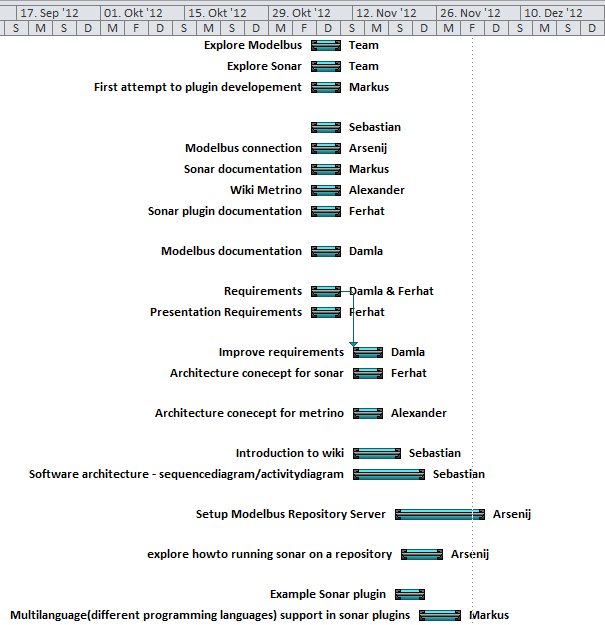
\includegraphics[width=\textwidth]{msp_part1}
\caption{Exercises - MS Project screenshot 1}
\end{center}
\end{figure}

\newpage

\begin{figure}[htb]
\begin{center}
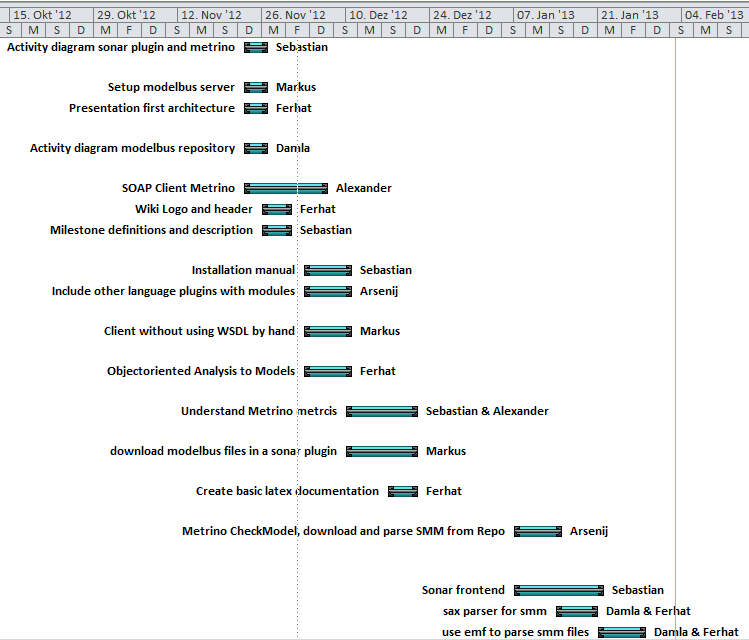
\includegraphics[width=\textwidth]{msp_part2}
\caption{Exercises - MS Project screenshot 2}
\end{center}
\end{figure}

\newpage

\begin{figure}[htb]
\begin{center}
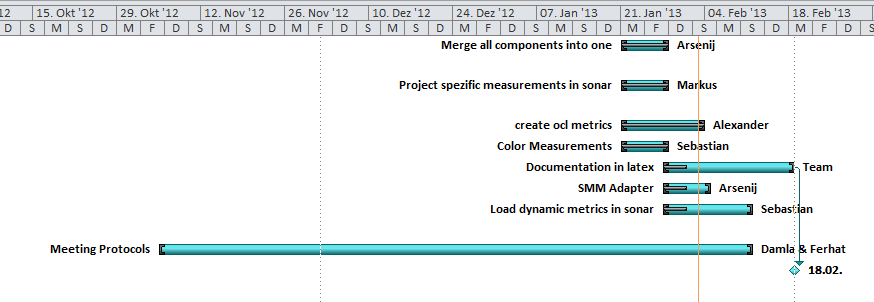
\includegraphics[width=\textwidth]{msp_part3}
\caption{Exercises - MS Project screenshot 3}
\end{center}
\end{figure}